%\chapter{Hybrid Physics-based Motion Control}
%\markboth{Hybrid Physics-based Motion Control}{Hybrid Physics-based Motion Control}
\chapter{Synthesis of Timpani Percussion Performances}
\markboth{Synthesis of Timpani Percussion Performances}{Synthesis of Timpani Percussion Performances}
\label{chapter:Synthesis}


%%%%%%%%%%%%%%%%%%%%%%%%%%%%%%%%%%%%%%%%%%%%%%%%%%%%%%%%%%%%%%%%%%%%%%%%%%%%%%%%%%%%%%%%%%%%%%%%%%%%%%%%%%%%%%%%%%%%

%Playing a musical instrument involves complex human behaviours. While performing, a skilled musician is able to precisely control his motion and to perceive both the reaction of the instrument to his actions and the resulting sound. This relationship between performer actions and the effects on the produced sound is crucial for understanding the mechanisms underlying musical learning or performance. Transposing these real-world experiences into virtual environments provides the possibility to explore novel solutions for designing virtual characters interacting with virtual musical instruments, and by extension for designing animated entities interacting with objects producing realistic sounds.\\

In this chapter, we propose a physically-based framework, in which a virtual character dynamically interacts with a physically simulated percussive instrument\footnote{The results presented in this chapter are the basis of the simulation platform documented at \href{http://www-valoria.univ-ubs.fr/Alexandre.Bouenard/index.php/Research/PhDThesis}{http://www-valoria.univ-ubs.fr/Alexandre.Bouenard/index.php/Research/PhDThesis}}. In particular, we present and evaluate a novel motion control paradigm for controlling a physical model of a virtual character, which is consistent with the analysis work presented in the previous chapter. We also propose an interaction scheme for controlling sound synthesis processes from this physically-based simulation framework for synthesizing virtual percussion performances.\\

The chapter is organized as follows. %First we introduce the motivation of the need of a novel motion control paradigm for the targetted application that is to synthesize virtual percussion performances (section \ref{sec:Synthesis_Introduction}).
We present an overview of the physical mechanisms occuring in our framework during the synthesis of virtual percussion performance in section \ref{sec:Synthesis_Overview}. The physics kernel including the physics modeling of the virtual percussionist as well as the novel motion control paradigm is presented and evaluated in section \ref{sec:Synthesis_Physics}. Section \ref{sec:Synthesis_Control} addresses the control of sound synthesis processes by the physical simulation of the virtual percussionist. Finally, section \ref{sec:Synthesis_Conclusion} concludes this work on the synthesis of virtual percussion performances.

%%%%%%%%%%%%%%%%%%%%%%%%%%%%%%%%%%%%%%%%%%%%%%%%%%%%%%%%%%%%%%%%%%%%%%%%%%%%%%%%%%%%%%%%%%%%%%%%%%%%%%%%%%%%%%%%%%%%


%%%%%%%%%%%%%%%%%%%%%%%%%%%%%%%%%%%%%%%%%%%%%%%%%%%%%%%%%%%%%%%%%%%%%%%%%%%%%%%%%%%%%%%%%%%%%%%%%%%%%%%%%%%%%%%%%%%%

%\section{Introduction and Motivation}
%\label{sec:Synthesis_Introduction}

%Virtual characters playing virtual musical instruments must interact in real-time with the sounding environment. Dynamic simulation is a promising approach to finely represent and modulate this interaction. Moreover, captured human motion can provide a database covering a large variety of gestures with various levels of expressivity. Three main problems have to be addressed in animating characters performing percussion gestures. First, physically-based simulations driven by motion capture data have to be considered, so that the physical interaction with the virtual world can be taken into account, and the generated movements can be driven by real examples. A second critical issue is the sound synthesis techniques which have to be used so that an effective mapping can be implemented between parameters generated from motion and sound synthesis parameters. Finally, the synchronization of different modalities and its use in interactive applications needs to be considered.\\

%Controlling adaptative and responsive virtual characters has been intensively investigated in \emph{Computer Animation} research. Among controller-based methods, most of the contributions have addressed the control of articulated figures using robotics-inspired proportionnal derivative (\emph{PD}) controllers \citeCGA{raibert86}. This has inspired many works for handling different types of motor tasks such as walking, running \citeCGA{hodgins:SIGGRAPH95}, composing these tasks \citeCGA{faloutsos:SIGGRAPH01} and easying the hard and time-consuming process of tuning such \emph{PD} controllers \citeCGA{allen:SCA07}.

%More related to our work are hybrid methods combining physics-based controllers and kinematic motion data, which aim at associating the advantage of user controllability of kinematics methods and the responsiveness of dynamics controllers. Our work is based on the tracking of motion capture data but differs from previous works by having a fully dynamically controlled character. 

%The specificity of our contribution lies also in the integration and the possible collaboration between \emph{IK} and \emph{ID} controllers, rather than handling strategies for transtionning between kinematic and dynamic controllers \citeCGA{zordan:SCA02, shapiro:PG03, zordan:TOG05}. We can also find in \citeCGA{zordan:CAS99} the use of \emph{IK} as a pre-process for modifying the original captured motion and simulating it on a different character anthropometry, we rather use \emph{IK} as a basis of our hybrid control method for specifying the control of a dynamic character from end-effector trajectories. This hybrid collaboration is particularly consistent for the synthesis of such ballistic motion that is percussion performance, which is not taken into account in related contributions \citeCGA{zordan:CAS99} \citeCM{bouenard:NIME08}.\\

%Alongside to the dynamic animation of virtual characters, physics-based sound synthesis methods have been widely studied, with the analogous goal of creating adaptative sounds towards changes in environment or objects properties. Since the introduction into the graphics community of modeling the surface vibrations of objects for sound synthesis \citeCM{vanDenDoel:ICAD96}, most of works have either focused on the direct use of vibrational modes \citeCM{obrien:SCA02} based on measurements \citeCM{corbett:Presence07}, or the simulation of surface vibrations using the finite element method \citeCM{obrien:SIGGRAPH01}. More recently, the high interest on modal synthesis has led to acceleration algorithms for handling large and complex environments \citeCM{bonneel:TOG08}.

%Our work involves in a similar manner physical models based on modal synthesis, but we point out to the difficulty of relating these sound synthesis schemes to their cause in the context of music performance, i.e. the instrumental gesture of a virtual performer. Here the focus is on the simulation of instrumental (percussion) gestures, as well as on the mapping between motion and sound synthesis.\\

%We therefore propose an architecture for physically exploring the interaction between motion and sound synthesis that eases the synchronization of different modalities and heterogenous data types (motion capture, motion simulation, sound control parameters). Previous works also involved a motion-driven approach for the synchronized generation of soundtracks from animations \citeCM{takala:SIGGRAPH92}. But as recalled in \citeCM{vanDenDoel:SIGGRAPH01}, despite many recent improvements, most of computer animation and simulation frameworks are still reluctant to integrate such synchronization method, moving therefore away from the interactive realism and presence that sound can give to computer animation applications. Our goal is to show how a physics modeling of the motion-sound interaction, combined with a carefully-designed system architecture can be of interest to that mean. Such a contribution has been proposed for haptic rendering systems \citeCM{avanzini:CAVW06, sinclair:IC08}, but to our knowledge it has not yet been exploited for the simulation and interaction of instrumental gestures with physics-based sound synthesis.

%%%%%%%%%%%%%%%%%%%%%%%%%%%%%%%%%%%%%%%%%%%%%%%%%%%%%%%%%%%%%%%%%%%%%%%%%%%%%%%%%%%%%%%%%%%%%%%%%%%%%%%%%%%%%%%%%%%%


%%%%%%%%%%%%%%%%%%%%%%%%%%%%%%%%%%%%%%%%%%%%%%%%%%%%%%%%%%%%%%%%%%%%%%%%%%%%%%%%%%%%%%%%%%%%%%%%%%%%%%%%%%%%%%%%%%%%

	\section{Overview}
	\label{sec:Synthesis_Overview}

The architecture of our system is presented in \myfigname \ref{fig:overview} and is made of two modules, allowing the physics simulation of percussion gestures to control sound synthesis processes. The first module includes a motion capture database used for driving a motion control policy model of a physics-based character. The second module expresses the interaction between the percussion motion simulation and the physics-based sound synthesis.\\

Concerning the motion control, the specificity of our contribution lies in the integration and the possible collaboration between inverse kinematics (\emph{IK}) and inverse dynamics (\emph{ID}) controllers, rather than handling strategies for transtioning between kinematic and dynamic controllers \citeCGA{shapiro:PG03, mandel:MsC04, zordan:TOG05}. We can also find in \citeCGA{zordan:CAS99} the use of \emph{IK} as a pre-process for modifying the original captured motion and simulating it on a different character anthropometry. We rather use \emph{IK} as a basis of our hybrid control method for specifying the control of a dynamic character from end-effector trajectories. This hybrid collaboration is particularly consistent for the synthesis of such ballistic motion that is percussion performance, which is not taken into account in related contributions \citeCGA{zordan:CAS99} \citeCM{bouenard:NIME08}.\\

Concerning the sound synthesis, our work involves physical models based on modal synthesis in a similar manner to recent works \citeCGA{raghuvanshi:I3D06, bonneel:TOG08}. However we point out to the difficulty of relating these sound synthesis schemes to their cause in the context of music performance, i.e. the instrumental gesture of a virtual performer. Here the focus is on the simulation of instrumental (percussion) gestures, as well as on the interaction between motion and sound synthesis.\\

\begin{figure}%[H]
	\centering
	\includegraphics[width=0.9\linewidth]{Chapters/5/Pics/Pdf/overview3.pdf}
%	\vspace{-0.5cm}
	\caption[System architecture and multimodal outputs]{System architecture and multimodal outputs. The {\it Physics-based Motion Control and Synthesis} step involves a {\it Motion Capture Database} and results in the {\it Visual Feedback}. The {\it Interaction} expresses the mapping between the percussion motion simulation and the {\it Sound Synthesis}, which results in the {\it Sound Feedback}.}
	\label{fig:overview}
\end{figure}

In addition, we propose an architecture to allow the synchronization of different modalities and heterogenous data types (motion capture, motion simulation, sound control parameters), as well as to enable the users to explore various interaction schemes between motion and sound simulations. Previous works also involved a motion-driven approach for the synchronized generation of soundtracks from animations \citeCM{takala:SIGGRAPH92}. But as recalled in \citeCM{vanDenDoel:SIGGRAPH01}, despite many recent improvements, most of computer animation and simulation frameworks are still reluctant to integrate such synchronization method, moving therefore away from the interactive realism and presence that sound can give to computer animation applications. Our goal is to show how a physics modeling of the motion-sound interaction, combined with a carefully-designed system architecture can be of interest to that mean. Such a contribution has been proposed for haptic rendering systems \citeCM{avanzini:CAVW06, sinclair:IC08}, but to our knowledge it has not yet been exploited for the simulation and interaction of instrumental gestures with physics-based sound synthesis.

%The first module includes a motion capture database used for driving a physics-based model of a virtual percussionist ("Instrumental Gesture Simulation" module). Section \ref{sec:Synthesis_Physics} details the modeling of the virtual percusionist as well as the underlying motion control paradigms involved in our novel hybrid motion control scheme.

%The second module expresses the interaction between the percussion motion simulation and the sound synthesis model ("Interaction" module). Section \ref{sec:Synthesis_Control} details the specially designed architecture for accelerating and easying this process. We recall that our interest lies more in the control of a sound synthesis model by the parameters extracted from the physics simulation of the virtual performer than the sound synthesis itself. As an example, we give in this section a derivation of this control step in the case of a modal model of a drum membrane.

%The specificity of our contribution lies in the integration and the possible collaboration between \emph{IK} and \emph{ID} controllers, rather than handling strategies for transtionning between kinematic and dynamic controllers \citeCGA{shapiro:PG03, mandel:MsC04, zordan:TOG05}. We can also find in \citeCGA{zordan:CAS99} the use of \emph{IK} as a pre-process for modifying the original captured motion and simulating it on a different character anthropometry, we rather use \emph{IK} as a basis of our hybrid control method for specifying the control of a dynamic character from end-effector trajectories. This hybrid collaboration is particularly consistent for the synthesis of such ballistic motion that is percussion performance, which is not taken into account in related contributions \citeCGA{zordan:CAS99} \citeCM{bouenard:NIME08}.

%Our work involves physical models based on modal synthesis in a similar manner to recent works \citeCGA{raghuvanshi:I3D06, bonneel:TOG08}. However we point out to the difficulty of relating these sound synthesis schemes to their cause in the context of music performance, i.e. the instrumental gesture of a virtual performer. Here the focus is on the simulation of instrumental (percussion) gestures, as well as on the interaction between motion and sound synthesis.

%We therefore propose an architecture for physically exploring the interaction between motion and sound synthesis that eases the synchronization of different modalities and heterogenous data types (motion capture, motion simulation, sound control parameters). Previous works also involved a motion-driven approach for the synchronized generation of soundtracks from animations \citeCM{takala:SIGGRAPH92}. But as recalled in \citeCM{vanDenDoel:SIGGRAPH01}, despite many recent improvements, most of computer animation and simulation frameworks are still reluctant to integrate such synchronization method, moving therefore away from the interactive realism and presence that sound can give to computer animation applications. Our goal is to show how a physics modeling of the motion-sound interaction, combined with a carefully-designed system architecture can be of interest to that mean. Such a contribution has been proposed for haptic rendering systems \citeCM{avanzini:CAVW06, sinclair:IC08}, but to our knowledge it has not yet been exploited for the simulation and interaction of instrumental gestures with physics-based sound synthesis.\\

%The architecture of our system is presented in \myfigname \ref{fig:overview} and is made of two modules, allowing the physics simulation of percussion gestures to control sound synthesis processes.

%The first module includes a motion capture database used for driving a physics-based model of a virtual percussionist ("Instrumental Gesture Simulation" module). Section \ref{sec:Synthesis_Physics} details the modeling of the virtual percusionist as well as the underlying motion control paradigms involved in our novel hybrid motion control scheme.

%The second module expresses the interaction between the percussion motion simulation and the sound synthesis model ("Interaction" module). Section \ref{sec:Synthesis_Control} details the specially designed architecture for accelerating and easying this process. We recall that our interest lies more in the control of a sound synthesis model by the parameters extracted from the physics simulation of the virtual performer than the sound synthesis itself. As an example, we give in this section a derivation of this control step in the case of a modal model of a drum membrane.

%%%%%%%%%%%%%%%%%%%%%%%%%%%%%%%%%%%%%%%%%%%%%%%%%%%%%%%%%%%%%%%%%%%%%%%%%%%%%%%%%%%%%%%%%%%%%%%%%%%%%%%%%%%%%%%%%%%%


%%%%%%%%%%%%%%%%%%%%%%%%%%%%%%%%%%%%%%%%%%%%%%%%%%%%%%%%%%%%%%%%%%%%%%%%%%%%%%%%%%%%%%%%%%%%%%%%%%%%%%%%%%%%%%%%%%%%

	\section{Physics-based Modeling and Motion Control}
	\label{sec:Synthesis_Physics}

The approach that we adopt for physically controlling percussion gestures from motion capture data is described in \myfigname \ref{fig:modelControl}.\\

It involves the physical modeling of a musculo-skeleton virtual percussionist from pre-recorded percussion performances, by merging the two kinematics ($\boldsymbol{T^K}$, \myequname \eqref{eq:kinRepresentation}) and dynamics ($\boldsymbol{T^D}$, \myequname \eqref{eq:dynRepresentation}) representations presented in section \ref{subsec:CA_VCM}.\\

Our novel motion control paradigm takes advantage of this double and complementary representation by the definition of a sensorimotor controller that tracks motion capture data according to two control modes. The first control scheme uses simple \emph{ID} controllers similarly to previous contributions \citeCGA{raibert86, hodgins:SIGGRAPH95, zordan:SCA02}, whereas the second mode involves a novel hybrid motion control scheme including a cascaded process of \emph{IK} and \emph{ID} controllers. This latter allows the control of the physical model of a virtual percussionist solely by specifying mallet extremity trajectories ($\boldsymbol{X_t}$).

\begin{figure}%[H]
	\centering
	\includegraphics[width=0.7\linewidth]{Chapters/5/Pics/Pdf/IK-ID-Control.pdf}
%	\vspace{-0.5cm}
	\caption[Physics-based modeling and control]{Physics-based modeling and control.}
	\label{fig:modelControl}
\end{figure}


		\subsection{Virtual Character Modeling}
		\label{subsec:Synthesis_Physics_VirtualCharacterModeling}


			\subsubsection{Representation and Anthropometry}
			\label{subsubsec:Synthesis_Physics_VirtualCharacterModeling_RepAnt}

The musculo-skeleton model of the virtual performer is composed of two skeleton layers, a dynamics layer ($\boldsymbol{T^D}$) and a kinematics layer ($\boldsymbol{T^K}$). It should be noted that this representation is not generic to any human anthropometry but specific to the simplified anthropometry initially recorded (cf. section \ref{sec:Analysis_MoCapDatabase}).\\

The dynamics skeleton $\boldsymbol{T^D}$ models the physical properties of the virtual character, and is composed of rigid bodies articulated by mechanical joints. Motion capture data of percussion performances are used to physically model and parameterize both the anthropometry and the mechanical joints of the virtual character, making a direct correspondence between the real performer and the virtual character. The physical properties of each rigid body composing the virtual character, such as mass, size of the limbs, density and inertia matrix are consistent with the anthropometry extracted from motion capture data, by using anthropometric tables \citeCGA{dempster:AJA67}.\\

The kinematics layer $\boldsymbol{T^K}$ of the virtual performer is composed of kinematics linear-angular position and velocity ($\boldsymbol{q}$, $\boldsymbol{\dot{q}}$) of joints articulating the rigid body composing $\boldsymbol{T^D}$. State features $\boldsymbol{q}$ and $\boldsymbol{\dot{q}}$ are namely obtained by the integration of the motion equations over time (\myequname \eqref{eq:physNewtonFormulation} for instance).


			\subsubsection{Joints}
			\label{subsubsec:Synthesis_Physics_VirtualCharacterModeling_Joints}

In addition, each mechanical joint has three rotational degrees of freedom, restricted to the angular limits of the human body, in order to avoid non realistic motion. Two formulations are available to extract the "lower" and "upper" limits of the angular joints, based on a statistical analysis of the motion capture data.\\

The first formulation uses the Euler angles representation, and computes basic statistical features to characterize joint limits. The singularity of this represention is however frequent (\emph{gimbal lock}), therefore we propose another formulation based on the quaternionic representation.\\

Following the approach of \citeCGA{johnson:PhD03}, we compute joint limits in the quaternion space\footnote{Thanks go to the developpers of the SMR library from the \href{http://www-valoria.univ-ubs.fr/SAMSARA}{\emph{VALORIA-SAMSARA}} lab, and particularly to N. Courty for helpful hints about the quaternion representation.}. The rotational (quaternionic) trajectory $\boldsymbol{Q}$ of a joint over time is transposed in the tangential space of its quaternionic mean $\bar{q}$, in which an SVD decomposition is applied. The resulting eigen values and axes ($\boldsymbol{\lambda}$, $\boldsymbol{e}$) are used for representing the motion distribution and for computing the joint limits by the specification of a bounding ellipsoid (\myalgname \ref{alg:quatSVD}).

\begin{algorithm}
	%\dontprintsemicolon
	\emph{}\;

	\begin{center}
		\begin{tabular}[3cm]{rcc}
			\multirow{1}{*}{In} & $\boldsymbol{Q} = \lbrace q_i, i \in [[1 \dots n]]\rbrace$ & Quaternionic time serie \\
			\\
			\multirow{1}{*}{Out} & $\lbrace \boldsymbol{\lambda}, \boldsymbol{e} \rbrace$ & Eigen values and axes \\
		\end{tabular}
	\end{center}
	\emph{}\;

	\emph{** Mean of $Q$ **}\;
	$\bar{q}$ = mean($\boldsymbol{Q}$)\;
 	\emph{}\;
 	
	\emph{** Transposition of the motion $Q$ in the tangent space of $\bar{q}$ **}\;
	$\boldsymbol{Q^{*}} = \log(\bar{q}*\boldsymbol{Q})$\;
	\emph{}\;

	\emph{** Eigen values and axes **}\;
	$\lbrace \boldsymbol{\lambda}, \boldsymbol{e} \rbrace = SVD(\boldsymbol{Q^{*}})$\;
	\emph{}\;

	\caption{Formulating joint limits in the quaternion space}
	\label{alg:quatSVD}
\end{algorithm}


		\subsection{Motion Control}
		\label{subsec:Synthesis_Physics_MotionControl}

Our approach to dynamic character control uses percussion gestures from a motion capture database, allowing to take into account all the variability and expressiveness of real percussion gestures. The variability can be due to various percussion performances using different mallet grips, various beat impact locations and several musical playing modes (see section \ref{sec:Analysis_MoCapDatabase}).\\

We propose two ways for achieving the motion control of the musculo-skeleton model (see \myfigname \ref{fig:motionSynthesis}), either by tracking motion capture data in the joint space (angular trajectories), or a novel hybrid motion control scheme for tracking end-effector trajectories in the 3D cartesian space. Tracking motion capture data in joint space requires \emph{ID} control, whereas tracking in the end-effector space requires both a cascaded collaboration of \emph{IK} and \emph{ID} controllers. In this latter case, the two inversion processes are strongly linked. 


			\subsubsection{\emph{ID} Motion Control}
			\label{subsec:Synthesis_Physics_MotionControl_InverseDynamics}

This control mode is related to motion capture data tracking by using \emph{ID} controllers. Angular trajectories ($\boldsymbol{\Theta_t}$) are first extracted from motion capture data, and used to drive the fully dynamically controlled virtual character. We use traditional proportional-derivative feedback controllers, modeled as damped springs and parameterized by manually-tuned damping and stiffness coefficients ($k_d$, $k_s$). Knowing the current state of the mechanical joint ($\boldsymbol{q}$, $\dot{\boldsymbol{q}}$) and the joint target ($\boldsymbol{q_t}$) to be reached, the torque ($\boldsymbol{\tau}$) is computed and exerted on the articulated rigid bodies, accordingly to \myequname \eqref{eq:equation1}.

\begin{equation}
	\boldsymbol{\tau} = k_s . (\boldsymbol{q_t} - \boldsymbol{q}) -  k_d . \dot{\boldsymbol{q}}
\label{eq:equation1}
\eqcaption{\emph{ID} control involved in the hybrid motion control}
\end{equation}

		\subsubsection{Hybrid Motion Control}
		\label{subsec:Synthesis_Physics_MotionControl_CartesianSpaceControl}

\begin{figure}%[H]
	\centering
	\includegraphics[width=0.9\linewidth]{Chapters/5/Pics/Pdf/hybridControl.pdf}
%	\vspace{-0.5cm}
	\caption[Hybrid physics-based motion control and synthesis]{Hybrid physics-based motion control and synthesis. The \emph{Motion Capture Database} is used for the physics modeling of the \emph{Virtual Character}, and for expressing two levels of \emph{Tracking}. These two levels allow the physics-based motion capture tracking, either in the \emph{Joint Space} from angular trajectories $\boldsymbol{q_t}$, or in the \emph{Cartesian Space} from end-effector trajectories $\boldsymbol{X_t}$. The hybrid control involves the combination of inverse kinematics (\emph{IK}) and inverse dynamics controllers (\emph{ID}).}
	\label{fig:motionSynthesis}
\end{figure}

A more intuitive physics control of the virtual character is proposed by combining \emph{IK} and \emph{ID} controllers. Instead of directly tracking angular trajectories from the motion capture database, this tracking mode consists in extracting end-effector positions in the 3D Cartesian space. From these Cartesian targets, an \emph{IK} method computes \myequname \eqref{eq:equation2} the kinematic postures (joint vector $\boldsymbol{q_t} $= \{$q_1$, ..., $q_n$\}), which are used as the desired input of the \emph{ID} controllers (\myalgname \ref{alg:hybridControl}), thus providing the required torques to control the physical character (\myfigname \ref{fig:motionSynthesis}).

\begin{equation}
	\begin{array}{l}
		\boldsymbol{\Delta q_t} = \mathcal{J}^{-1}(\boldsymbol{q}).(\boldsymbol{X_t} - \boldsymbol{X}), \hspace{2mm} \boldsymbol{q_t} = \boldsymbol{q} + \boldsymbol{\Delta q_t} \\
		\boldsymbol{\tau} = k_s . (\boldsymbol{q_t} - \boldsymbol{q}) -  k_d . \dot{\boldsymbol{q}}
	\end{array}
\label{eq:equation2}
\eqcaption{\emph{IK} control involved in the hybrid motion control}
\end{equation}

\begin{algorithm}[H]
	%\dontprintsemicolon
	\emph{}\;

	\begin{center}
		\begin{tabular}[3cm]{rcc}
			\multirow{2}{*}{In} & $\boldsymbol{AC} = \lbrace \boldsymbol{T^K}, \boldsymbol{T^D}\rbrace$ & Articulated chain \\
				& $F_T$ & Task frequency\\
				& $F_S$ & Simulation frequency\\
				& $\boldsymbol{q}, \boldsymbol{\dot{q}}$ & Current kinematic posture of $T^K$ \\
				& $\boldsymbol{X}$ & Current end-effector position of $T^K$ \\
				& $\boldsymbol{X_t}$ & Targetted end-effector position of $T^K$ \\
			\\
			\multirow{3}{*}{Out} & $\boldsymbol{\mathcal{J}}$ & Jacobian matrix \\
				& $\boldsymbol{q_t}$ & Targetted kinematic posture of $T^K$ \\
				& $\boldsymbol{\tau}$ & Resulting torques to be exerted on $T^D$ \\
		\end{tabular}\;
	\end{center}

	\While{Read task at $F_T$}{
		\emph{}\;
		$\boldsymbol{X_t}$ $\leftarrow$ New mallet extremity\;
		\emph{}\;

		$numIKID$ = 0\;
		\emph{}\;

		\For{numIKID < $F_S$/$F_T$}{
			\emph{}\;
			\emph{** Inverse Kinematics **}\;
			$\boldsymbol{\mathcal{J}}$ $\leftarrow$ ComputeJacobian($\boldsymbol{T^K}$, $\boldsymbol{q}$)\;
			$\boldsymbol{q_t}$ $\leftarrow$ InverseKinematics($\boldsymbol{\mathcal{J}}$, $\boldsymbol{X}$, $\boldsymbol{X_t}$, $\boldsymbol{q}$)\;
			\emph{}\;
	
			\emph{** Inverse Dynamics **}\;
			$\boldsymbol{\tau}$ $\leftarrow$ InverseDynamics($\boldsymbol{q}$, $\boldsymbol{\dot{q}}$, $\boldsymbol{q_t}$)\;
			\emph{}\;
	
			\emph{** Update **}\;
			ApplyTorques($\boldsymbol{T^D}$, $\boldsymbol{\tau}$)\;
			Update($\boldsymbol{T^K}$, $\boldsymbol{T^D}$)\;
		\emph{}\;
		}
	}
	\emph{}\;

	\caption{Hybrid motion control combining \emph{IK} and \emph{ID} controllers}
	\label{alg:hybridControl}
\end{algorithm}

$\mathcal{J}$ represents the Jacobian of the system to be controlled, $\boldsymbol{X}$ and $\boldsymbol{X_t}$ represent respectively the current and target end-effector positions in the Cartesian space. The modularity of the presented approach for combining \emph{IK} and \emph{ID} controllers allows to consider any method, so that our system supports at the momemt several \emph{IK} formulations (transpose, pseudo-inverse and damped-least-squares, see section \ref{subsubsubsec:CA_MC_Kinematics_Inv}) that can be combined with simple \emph{ID} formulations. One may equally use other \emph{IK} techniques, such as learning techniques described in \citeCGA{gibet:CASA03, gibet:ISDA07}.

\myalgname \ref{alg:hybridControl} shows the principle of the hybrid motion control, composed of two nested loops. The first one concerns the task specification (mallet extremity position). Between two task updates, the second loop involves the cooperation of the \emph{IK} and \emph{ID} formulations. For example, for a task frequency of 250 Hz and a simulation frequency of 10000 Hz, the second simulation loop is called 10000/250=40 times, which can be sufficient  so that the \emph{IK} algorithm converges, and consequently ending with the \emph{ID} convergence.\\

Using such an \emph{IK} formulation necessitates the computation of the Jacobian matrix, and therefore we defined an equivalent representation of the articulated chain, both in the kinematics and dynamics spaces. The main difficulty with the coupling of both kinematics and dynamics controllers is that the convergence of the \emph{IK} algorithm is added to the difficulty of tuning the parameters of the \emph{PD} dynamic controllers. But this approach enables the manipulation of motion capture data in the 3D Cartesian space (configuration $\boldsymbol{X_t}$) instead of the angular space ($\boldsymbol{q_t}$), which is more consistent and intuitive for controlling percussion gestures, by using end-effector trajectories, for instance mallets extremities.\\


		\subsection{Results}
		\label{subsec:Synthesis_Physics_Results}

%		\subsubsection{Methodology}
%		\label{subsubsec:Synthesis_Physics_Results_Methodo}

%The physical model of the virtual character is composed of 19 joints, totalling 57 degrees of freedom. The Open Dynamic Engine \citeCGA{ode} is used for the overall motion simulation. Masses, inertia, limb lengths, as well as joint limits are estimated from real percussion performers. Concerning the hybrid control mode, different inverse kinematics methods may be combined to \emph{ID} controllers. These results use an implenentation of the Damped Least Squares method \citeCGA{wampler:SMC86}, a simple yet more robust adaptation of the pseudo-inverse regarding the singularity of the inverse kinematics problem.

%It should be noted that in all results described in the following points, we kept the same parameterization of the damped springs of the virtual character.\\

%A qualitative evaluation of the presented hybrid motion control is first conducted. The results obtained by the two tracking modes used to physically control the virtual percussionist are compared: a) motion capture tracking in joint space, involving only \emph{ID} controllers, and b) motion capture hybrid tracking in cartesian space, involving a combination of \emph{IK} and \emph{ID} controllers.\\

%Then a more quantitative evaluation is presented for quantifying the errors made by the two motion tracking modes during the simulation of various types of percussion gestures. An evaluation directed by a classification/recognition methodology analogous to chapter \ref{chapter:Analysis} is also conducted.

The physical model of the virtual character is composed of 17 joints, totalling 51 degrees of freedom. The Open Dynamic Engine \citeCGA{ode} is used for the forward dynamics simulation of the motion equations. Masses, inertia, limb lengths, as well as joint limits are estimated from real percussion performers. Concerning the hybrid control mode, many inverse kinematics methods may be involved in our cascaded control mode. These results have been obtained using an implementation of the damped-least-squares method \cite{wampler:SMC86}, a simple yet more robust adaptation of the pseudo-inverse regarding the singularity of the inverse kinematics problem. The hybrid control scheme presented previously is tested on the control of the two arms of the virtual character, tracking a sequence of percussion gestures for synthesizing whole arm movements only from the specification of the mallet extremity trajectories.

The results presented in this section compare the traditional \emph{ID} control mode to our hybrid control scheme. It should be noted that for making such a comparison possible, the parameters that can change drastically the resulting simulations have been kept constant. Such parameters include for instance the simulation rate, the recorded motion to be simulated as well as the parameterization of the damped springs composing the dynamic layer of the virtual character.\\

A qualitative evaluation of the presented hybrid motion control is first conducted. The results obtained by the two tracking modes used to physically control the virtual percussionist are compared: a) motion capture tracking in joint space, involving only \emph{ID} controllers, and b) motion capture hybrid tracking in Cartesian space, involving the cascaded combination of \emph{IK} and \emph{ID} controllers. In a second time, we quantitatively evaluate the two tracking modes by quantifying the errors made during the simulation of various types of percussion gestures in each control case. An evaluation directed by a classification/recognition methodology analogous to chapter \ref{chapter:Analysis} is also conducted.\\

%Then a more quantitative evaluation is presented for quantifying the errors made by the two motion tracking modes during the simulation of various types of percussion gestures. An evaluation directed by a classification/recognition methodology analogous to chapter \ref{chapter:Analysis} is also conducted.\\

Concerning the quantitative evaluation, a critical issue to consider is the metric used for evaluating the effectiveness of our hybrid solution compared to traditional \emph{ID} control. A few works have addressed the question of the user sensibility to various motion metrics \citeCGA{reitsma:TOG03, ren:TOG05}. In this work, the ballistic nature of percussion motion makes it however easy to conduct an extensive evaluation by focusing on mallet extremity trajectories. We also show that our solution leads to a coherent motion in the joint space for specific degrees of freedom that are shown to be of paramount importance in percussion playing.


			\subsubsection{Qualitative Evaluation}
			\label{subsubsec:Synthesis_Physics_Results_QualitativeEval}

%For this qualitative evaluation, we ran the simulation of a set of pre-recorded percussion gestures (\emph{French} grip, \emph{legato}). \myfigname \ref{fig:mocapIKIDEvaluation} compares raw data from captured motion with the two modes of control (\emph{ID} only, and the hybrid combination of \emph{IK} and \emph{ID}).\\

%The hybrid control scheme tracks one percussion gesture for synthesizing whole arm movements only from the specification of the tip of the mallets trajectories. \myfigname \ref{fig:mocapIKIDEvaluation} (top) presents the comparison between raw motion capture data and data generated by the \emph{IK} process. It shows that data generated by the \emph{IK} formulation are consistent with real ones, especially for the elbow flexion angle that is one of the most important degree of freedom of the arm in percussion gestures (especially during preparatory phases \citeIPA{bouenard:ENACTIVE08}).\\
 
%We finally present the comparison of the two control modes (\emph{ID} control only and hybrid control) in \myfigname \ref{fig:mocapIKIDEvaluation} (bottom). One interesting issue is the accuracy of the hybrid control mode compared to the simple \emph{ID} control. This observation lies in the fact that the convergence of motion capture tracking is processed in the joint space in the case of \emph{ID} control, adding and amplifying multiple errors on the different joints and leading to a greater error than processing the convergence in the Cartesian space for the hybrid control.\\

%Although such cascaded chain of \emph{IK} and \emph{ID} controllers run in real-time, the main drawback of this improvement is however the additional computationnal cost of the \emph{IK} algorithm which is processed at every simulation step. It provides nevertheless a more flexible motion edition technique for controlling a fully physics-based virtual character, that eases the co-articulation between successive motion units. %This is illustrated in \myfigname \ref{fig:impro}, which shows the creation of a gesture score from a musical score, and the animation of the virtual percusionist following this score.

For this qualitative evaluation, we ran the simulation of a set of pre-recorded percussion gestures (\emph{French} grip, \emph{legato}). Figure \ref{fig:mocapIKIDEvaluation} compares raw data from captured motion with the two modes of control (\emph{ID} only, and the hybrid combination of \emph{IK} and \emph{ID}).\\

\begin{figure}%[H]
	\begin{center}
		\subfigure[]{\label{fig:mocapIKIDEvaluation1}\includegraphics[width=0.45\linewidth]{Chapters/5/Pics/Pdf/wrist_angle2.pdf}}
		\hspace{6mm}
		\subfigure[]{\label{fig:mocapIKIDEvaluation4}\includegraphics[width=0.45\linewidth]{Chapters/5/Pics/Pdf/drumstick_pos.pdf}}\\
		\subfigure[]{\label{fig:mocapIKIDEvaluation2}\includegraphics[width=0.45\linewidth]{Chapters/5/Pics/Pdf/elbow_angle.pdf}}
		\hspace{6mm}
		\subfigure[]{\label{fig:mocapIKIDEvaluation5}\includegraphics[width=0.45\linewidth]{Chapters/5/Pics/Pdf/wrist_pos.pdf}}\\
		\subfigure[]{\label{fig:mocapIKIDEvaluation3}\includegraphics[width=0.45\linewidth]{Chapters/5/Pics/Pdf/shoulder_angle.pdf}}
		\hspace{6mm}
		\subfigure[]{\label{fig:mocapIKIDEvaluation6}\includegraphics[width=0.45\linewidth]{Chapters/5/Pics/Pdf/elbow_pos.pdf}}
	\end{center}
	\vspace{-0.6cm}
	\caption[Comparison of captured and simulated trajectories]{Comparison of captured and simulated trajectories using the two motion control schemes: (a), (c) and (e) resp. for wrist, elbow and shoulder flexion angles, (b), (d) and (f) resp. for mallet, wrist and elbow height positions.}
	\label{fig:mocapIKIDEvaluation}
\end{figure}

\myfigname \ref{fig:mocapIKIDEvaluation1}, \ref{fig:mocapIKIDEvaluation2} and \ref{fig:mocapIKIDEvaluation3} present the comparison between raw motion capture data and data generated by the two control modes for wrist, elbow and shoulder flexion angle trajectories. These results show that data generated by the \emph{IK} involved in the hybrid control mode are consistent with real ones, especially for wrist and elbow trajectories. Data generated by our hybrid solution is more accurate compared to \emph{ID} control, this latter shows indeed a motion exaggeration that tends to be avoided by our solution.

More specifically about shoulder flexion angle, \myfigname \ref{fig:mocapIKIDEvaluation3}, it seems that the \emph{IK} process looses the pattern of the original motion, while leading to more accurate extrema occuring at beat impacts compared to \emph{ID} control. This loss is however of lower importance in percussion gestures, as attested in \cite{bouenard:ENACTIVE08} where it is argued that wrist and elbow angle trajectories are one of the most important degrees of freedom in percussion arm mechanisms.\\
 
We also present the result comparison of the two control modes concerning height trajectories for the mallet extremity, wrist and elbow in \myfigname \ref{fig:mocapIKIDEvaluation4}, \ref{fig:mocapIKIDEvaluation5} and \ref{fig:mocapIKIDEvaluation6}. One interesting issue is the accuracy of the hybrid control mode compared to the simple \emph{ID} control. The motion exaggeration observed previously in joint flexion trajectories in the case of \emph{ID} control is propagated on joint position trajectories. Conversely, our hybrid solution leeds to a more accurate tracking in joint position trajectories. This observation lies in the fact that the convergence of motion capture tracking is processed in the joint space in the case of \emph{ID} control, adding and amplifying multiple errors on the different joints and leading to a greater error than processing the convergence in the Cartesian space for the hybrid control.

One limitation however arises in elbow position trajectories. While the \emph{ID} control mode results again in an amplified motion, our hybrid control solution results in a loss in the motion pattern of original data. The elbow position trajectory resulting from the hybrid control mode leads to a more stiff and somewhat constant motion. This can be related to the inverse kinematics scheme which does not include any secondary goals, as already pointed out in \citeCGA{klein:TSMC83}. This may be explained also by the fact that the \emph{IK} algorithm favorizes the accuracy of the most distal joints compared to joints at the basis of the articulated chain. Another reason to this limitation could be the influence of the physics simulation on the convergence of the inverse kinematics scheme.\\

Although such cascaded chain of \emph{IK} and \emph{ID} controllers runs in real-time, the main drawback of this improvement is however the additional computationnal cost of the \emph{IK} algorithm which is processed at every simulation step. It provides nevertheless a more flexible motion edition technique for controlling a physics-based virtual character solely by end-effector trajectories. It also provides a consistent control scheme as regards to the preliminary analysis conducted in chapter \ref{chapter:Analysis}.

%\newpage
%\vfill

%\begin{figure}[H]
%	\centering
%	\includegraphics[width=\linewidth]{Chapters/5/Pics/Pdf/MoCap_IK_Comparison.pdf}
%	\includegraphics[width=\linewidth]{Chapters/5/Pics/Pdf/MoCap_ID_IKID_Comparison.pdf}
%	\caption[Comparison of captured and simulated mallet trajectories for a \emph{legato} stroke]{Comparison of captured and simulated mallet trajectories for a \emph{legato} stroke, using the two motion control schemes. Top: comparison of elbow flexion angle trajectories, original motion data (plain) vs. data generated by the \emph{IK} algorithm (dash). Bottom: comparison of mallet trajectories, original motion capture data (plain) vs. joint space (\emph{ID}) physics tracking (little dash) vs. cartesian space (\emph{IK} + \emph{ID}) physics tracking (large dash).}
%	\label{fig:mocapIKIDEvaluation}
%\end{figure}


			\subsubsection{Quantitative Evaluation}
			\label{subsubsec:Synthesis_Physics_Results_QuantitativeEval}

%An extensive evaluation of the two control modes is presented in \myfigname \ref{fig:rms}. This takes into account the test of the two control algorithms on 200 simulation trials for various gesture variations (from top to bottom: \emph{legato}, \emph{tenuto}, \emph{accent}, \emph{vertical accent} and \emph{staccato}). For each simulation trial, the root mean square error and standard deviation is processed compared to a gesture unit initially chosen in the motion capture database.\\

%From these results, one can easily conclude that the cascaded hybrid combination of \emph{IK} and \emph{ID} controllers leads to a more accurate minimization of the error commited on mallet extremity trajectories of about 1 centimeter, compared to simple \emph{ID} controllers. The standard deviation along simulation trials are also more minimized for the hybrid motion paradigm compared to the \emph{ID} control.

An extensive evaluation of the two control modes is presented in \myfigname \ref{fig:rms}. This takes into account the test of the two control algorithms on 200 simulation trials for various playing modes (from top to bottom: \emph{legato}, \emph{tenuto}, \emph{accent}, \emph{vertical accent} and \emph{staccato}). \myfigname \ref{fig:playingModes} shows examples of longitudinal-vertical phases of the mallet extremity position for each playing mode. This emphasizes that these playing modes present drastically different gesture dynamics in mallet motion, especially regarding its longitudinal and vertical amplitude. Each simulation trial corresponds to a gesture unit that is simulated according to the two control modes. The root mean square error and its standard deviation are processed as regards to the mallet extremity compared to the corresponding motion initially chosen in the motion capture database.\\

From the results presented in \myfigname \ref{fig:rms}, one can easily conclude that the cascaded hybrid combination of \emph{IK} and \emph{ID} controllers leads to a more accurate minimization of the error commited on mallet extremity trajectories of about 1 centimeter, compared to simple \emph{ID} controllers. The standard deviation along simulation trials are also more minimized for the hybrid motion paradigm compared to the \emph{ID} control.\\ %Such a difference of 1 centimeter in the average errors between the two control modes can be considered as negligeable. However the mallet extremity informations around the beat impacts can change drastically the nature of the resulting sounds.\\

\begin{figure}[H]
	\begin{center}
		\includegraphics[width=\linewidth]{Chapters/5/Pics/Pdf/RMSE-RMSD.pdf}
	\end{center}
	\vspace{-0.5cm}
	\caption[Comparison of RMS errors between captured and simulated mallet trajectories for various playing modes]{Comparison of RMS errors between captured and simulated mallet trajectories for various playing modes, using the two motion control schemes: \emph{ID} (point line) and \emph{IK + ID} (plain). For each playing mode (from top to bottom: \emph{legato}, \emph{tenuto}, \emph{accent}, \emph{vertical accent} and \emph{staccato}), Root Mean Square Error (RMS-E, black) and Standard Deviation (RMS-SD, red) are computed on 200 simulation trials.}
	\label{fig:rms}
\end{figure}

It should be noted that this average difference of 1 centimeter of accuracy cannot be considered as negligeable, since the sound synthesis model taking mallet extremity informations around the beat impacts can change drastically the nature of the resulting sounds. For instance, in the case of modal sound synthesis models, the accuracy of mallet extremity trajectories is of paramount importance since it will change the selection of the excited mode shapes.\\

Another evaluation method has been considered for insuring the accuracy of the hybrid motion control scheme. In an analous manner to the evaluation of percussion playing characteristics in chapter \ref{chapter:Analysis}, a classification/recognition methodology has been adopted. A SVM classifier with RBF kernel functions has been trained with the extracted parameters described in section \ref{sec:Analysis_TimpaniAnalysis} from motion capture data, thus forming the training set. These gesture characteristics have also been extracted from the 200 simulations trials, which are this time forming the query set. The results of the classification/recognition of simulated playing modes (\emph{legato}, \emph{tenuto}, \emph{accent}, \emph{vertical accent} and \emph{staccato}) are summarized in the confusion matrix in \mytabname \ref{tab:recognitionFrenchVariationsSim}.
 
\begin{table}%[H]
	\centering
	\caption[SVM recognition of simulated \emph{French} grip playing modes]{SVM recognition of simulated \emph{French} grip playing modes (in percentage of success) using the combination of mallet velocity and acceleration extrema presented in Fig. \ref{fig:classifParameters}}
	\vspace{2mm}
	\begin{tabular}{||x{1.9cm}||x{1.9cm}|x{1.9cm}|x{1.9cm}|x{1.9cm}|x{1.9cm}||} \hline
		\small{$Training$ / $Test$} & \small{$Legato$} & \small{$Tenuto$} & \small{$Accent$} & \small{$V.Accent$} & \small{$Staccato$}		\tabularnewline \hline \hline
		\small{$Legato$} & 		\small{\textbf{92.6}} & \small{4.8} & \small{0} & \small{2.6} & \small{0} 	\tabularnewline \hline
		\small{$Tenuto$} & 		\small{3.7} & \small{\textbf{94.2}} & \small{1.2} & \small{0.9} & \small{0}	\tabularnewline \hline
		\small{$Accent$} & 		\small{2.5} & \small{0} & \small{\textbf{96.4}} & \small{0} & \small{1.1}	\tabularnewline \hline
		\small{$V.Accent$} & 	\small{0.5} & \small{0.6} &	\small{0} & \small{\textbf{93.9}} & \small{4.7}	\tabularnewline \hline
		\small{$Staccato$} & 	\small{0} & \small{0} & \small{0.5} & \small{4.4} & \small{\textbf{95.1}}	\tabularnewline \hline
	\end{tabular}
	\label{tab:recognitionFrenchVariationsSim}
\end{table}

These results attest the consistency of the novel hybrid motion control scheme presented in this section, giving an average recognition rate of more than 94{\%} of success for the simulated playing modes.


		\subsection{Conclusion}
		\label{subsec:Synthesis_Physics_Conclusion}

We presented in this section the derivation of the modeling and motion control of a physical model of a virtual performer which has the particularity of merging two complementary (kinematics and dynamics) representations. We also derived consequently a novel hybrid motion control scheme dedicated to percussion gestures that allows the control of the physical virtual performer solely by the specification of mallet extremity trajectories. We have particularly shown that this hybrid motion control can be more effective than simple \emph{ID} controllers for percussion gestures. Moreover, in an edition step, managing the control of a physical model only by 3D Cartesian targets is more convenient than handling whole kinematic postures.\\

From a musical point of view, and according to the conclusions of the analysis study conducted in chapter \ref{chapter:Analysis}, such an hybrid motion control scheme is also more consistent than \emph{ID} control as regards to percussion tasks, since our hybrid control scheme only needs the specification of mallet extremity trajectories. In the next section, we focuse on the interaction between motion and sound simulations (\myfigname \ref{fig:overview}) so that the simulated percussion actions of the virtual performer can influence the sound production process.

%%%%%%%%%%%%%%%%%%%%%%%%%%%%%%%%%%%%%%%%%%%%%%%%%%%%%%%%%%%%%%%%%%%%%%%%%%%%%%%%%%%%%%%%%%%%%%%%%%%%%%%%%%%%%%%%%%%%


%%%%%%%%%%%%%%%%%%%%%%%%%%%%%%%%%%%%%%%%%%%%%%%%%%%%%%%%%%%%%%%%%%%%%%%%%%%%%%%%%%%%%%%%%%%%%%%%%%%%%%%%%%%%%%%%%%%%

	\section{Interaction between Motion and Sound Synthesis}
	\label{sec:Synthesis_Control}

We propose a general architecture (\myfigname \ref{fig:interaction}) that allows to simultaneously and asynchronously run the physics simulation of percussion gestures, graphics and sound rendering processes, as well as to handle their interaction in real-time. This architecture is effective for managing different modalities and data types, and for specifying at the physics level the interaction between these former.

	\subsection{Asynchronous Client-Server Architecture}
	\label{subsec:Synthesis_Control_InteractionArchitecture}

\begin{figure}
	\centering
	\includegraphics[width=\linewidth]{Chapters/5/Pics/Pdf/interaction2.pdf}
%	\vspace{-0.5cm}
	\caption[Asynchronous server-client architecture of our system]{Asynchronous server-client architecture of our system.}
	\label{fig:interaction}
\end{figure}

Our system makes possible the multimodal integration, interaction and synchronization of visual and sounding media, and is composed of four components represented as physics, graphics, interaction and sound managers.\\

Multimodal processes such as graphics and sound rendering are fundamently different, and achieving a real-time interaction between both of them can be hazardous. The first difficulty that appears when managing such media is their discrepency in time constants: graphics rendering is usely admitted effective at about 33Hz, whereas sound rendering needs a higher time sample ate around 44kHz. Moreover, the graphics rendering is the visible layer of a far more demanding process that is the physics simulation, requiring the handling of two other different time rates since our method relies on motion capture tracking: the original motion capture time rate and the time step of the physics simulation. An approach could consist in running synchronously every manager at the sound rate, but such an approach would fall short in real-time considerations.\\

We therefore propose an asynchronous client-server scheme for handling the interaction between the physics, graphics and sound managers. This enables the possible distribution of the different managers on distinct platforms, thus reducing the computational cost of each manager and its impact on the others.

For this purpose, we define a communication layer between the managers, based on the  Open Sound Control (\emph{OSC}) communication protocol. The \emph{OSC} protocol has been primarly designed to enable the networking and interoperability between interactive computer music applications \citeCGA{wright:OS05}. Its scheme is based on a ''transport-independant'' server-client relationship, supporting any network technology (ethernet or wireless, UDP or TCP/IP) and serial connection. Similarly to MIDI, the \emph{OSC} scheme is based on the interaction of communicative points and assigns values to these. OSC differs fondamuntally from MIDI in handling namespaces, data types and time retrieval. \emph{OSC} features intuitive naming and adressing rules (on the contrary to MIDI byte encoding), as well as an extended set of adresses and namespaces (compared to the limited and limiting six channels of MIDI). \emph{OSC} allows also the transmission of any type of structure of any size, even MIDI data, providing a standard for many software or hardware developpments. Eventually, \emph{OSC} features message time tagging for managing priority and anticipating future events. For a complete derivation of \emph{OSC} principles and functionalities, readers are refered to \citeCM{wright:NIME03, freed:NIME09, osc}.
		
The asynchronous exchange of data is materialized here by the interaction between the output of motion synthesis and the input of sound synthesis. Events produced during the physical simulation are dealt by the interaction module which feeds the sound synthesis processes and the visual outputs.


		\subsection{Motion-Sound Physics Interaction}
		\label{subsec:Synthesis_Control_InteractionMapping}

For sound synthesis, we consider in our work the modal synthesis technique. Note however that the modularity of our system allows to plug any sound synthesis model to the instrumental gesture simulation. Modal synthesis is an efficient way of representing the vibrations of resonating objects as the motion simulation of systems composed of masses connected with springs and dampers (cf. section \ref{subsubsubsec:CM_SS_Physics_SO}). This physically-based approach enables the direct modeling of the contact force impact and its effect on mode shapes. According to \citeCM{avanzini:ICMC01}, this force depends on the state (displacement and velocity) of the colliding modal objects.

We define in this section a practical interaction between the instrumental gesture simulation and a modal model of a drum membrane. Let us suppose first that such a model is available, and consider a slightly modified version of the model derived in appendix \ref{sec:ssDerivation:mM} for taking into account an interaction force on the drum membrane.
The model is governed by the motion of $N$ coupled oscillators, that can be excited by a force $\boldsymbol{f}$, \myequname \eqref{eq:equation3}.

\begin{equation}
	\boldsymbol{M} . \ddot{\boldsymbol{z}}(t) + \boldsymbol{K} . \boldsymbol{z}(t) = \boldsymbol{f}
\label{eq:equation3}
\eqcaption{Modal synthesis formulation under the influence of an external force}
\end{equation}

The factorization of the problem considers a solution of the form $\boldsymbol{z}(t) = \boldsymbol{s} . \sin(\omega.t + \phi)$ where $\boldsymbol{s}$ are again refered as the \emph{modal shapes} of the system. This leads to the equivalent normal formulation of the problem in the orthogonal basis made of the mode shapes, \myequname \eqref{eq:equation4} (see appendix \ref{sec:ssDerivation:mM} for intermediate steps).

\begin{equation}
	\begin{array}{l}
		\boldsymbol{M}_S . \ddot{\boldsymbol{q}}(t) + \boldsymbol{K}_S . \boldsymbol{q}(t) = \boldsymbol{S}^T . \boldsymbol{f} \\
		with\ \boldsymbol{S} = [s_1, ..., s_N],\ \boldsymbol{z} = \boldsymbol{S} . \boldsymbol{q},\ \boldsymbol{M}_S = \boldsymbol{S}^T . \boldsymbol{M} . \boldsymbol{S}\ and\ \boldsymbol{K}_S = \boldsymbol{S}^T . \boldsymbol{K} . \boldsymbol{S}
	\end{array}
\label{eq:equation4}
\eqcaption{Modal synthesis formulation under the influence of an external force: normal formulation}
\end{equation}

\myequname \eqref{eq:equation4} shows explicitly that the \emph{modal shapes} of the system (matrix $\boldsymbol{S}$) defines how the external force $\boldsymbol{f}$ acts on the modes. As an illustration, an external force acting only on the j$^{th}$ mass of the model is transmitted to the i$^{th}$ mode by a scaling factor $s_{i, j}$ (the modal shape of the i$^{th}$ mode at the j$^{th}$ mass node). If the i$^{th}$ mode has a shape that contains the j$^{th}$ mass node of the model, then the scaling factor $s_{i, j}$ is null, and finally no force is "applied" to this mode. According to \myequname \eqref{eq:equation4}, the vertical oscillation of the j$^{th}$ mass of the model can be written as $z_j(t) = \sum_{i = 1}^{N} s_{i, j} . q_i(t)$, such that if the i$^{th}$ mode has a node at the j$^{th}$ mass this mode will not be heard at that listening point.\\

The interaction manager includes a collision detection algorithm (\myfigname \ref{fig:interaction}) that can retrieve the physical features of any contact event produced when the drum is excited during the instrumental gesture simulation. In particular, it provides information on the impact position, velocity and force (direction and amplitude), which can be related to the previously presented inputs to a modal model of a drum membrane according to a direct one-to-one mapping.


		\subsection{Results}
		\label{subsec:Synthesis_Control_Results}

Our software architecture makes use of the \emph{OSC} protocol, without any assumption about the hosting of OSC clients and servers, making it possible to run the graphics, physics and sound managers on distinct computers. This architecture has been successfully tested by running the graphics/physics and sound cores on two different platforms linked by an ethernet connexion, providing an effective and reliable communication between the two.

As for the sound synthesis system, a modal model of a drum membrane has been designed\footnote{Thanks to the help of Nicholas Ellis from \emph{IRCAM}, who designed the overall modal model of the drum membrane.} using the \emph{Modalys} framework \citeCM{adrien:PhD89, adrien91, ellis:ICMC05}. It allows the real-time parameterization of the membrane properties (size, mass, tension), as well as the parameters of the modal synthesis (number of modes, resonances), thus rendering varied sound feedback effects. The impact location and force on the drum membrane can also be parameterized, offering a real-time sound rendering in response to an instrumental gesture simulation.

The user interface presented in \myfigname \ref{fig:userInterface} was implemented using Pure Data \citeCM{puckette:ICMC96}, which is considered as the sound OSC server in our architecture. It shows how users can instantiate and access OSC components (top control panels) by modifying, creating and registering new interaction messages between the physics (left control panel), graphics (middle control panel) and sound (right control panel) managers.

\begin{figure}[H]
	\centering
	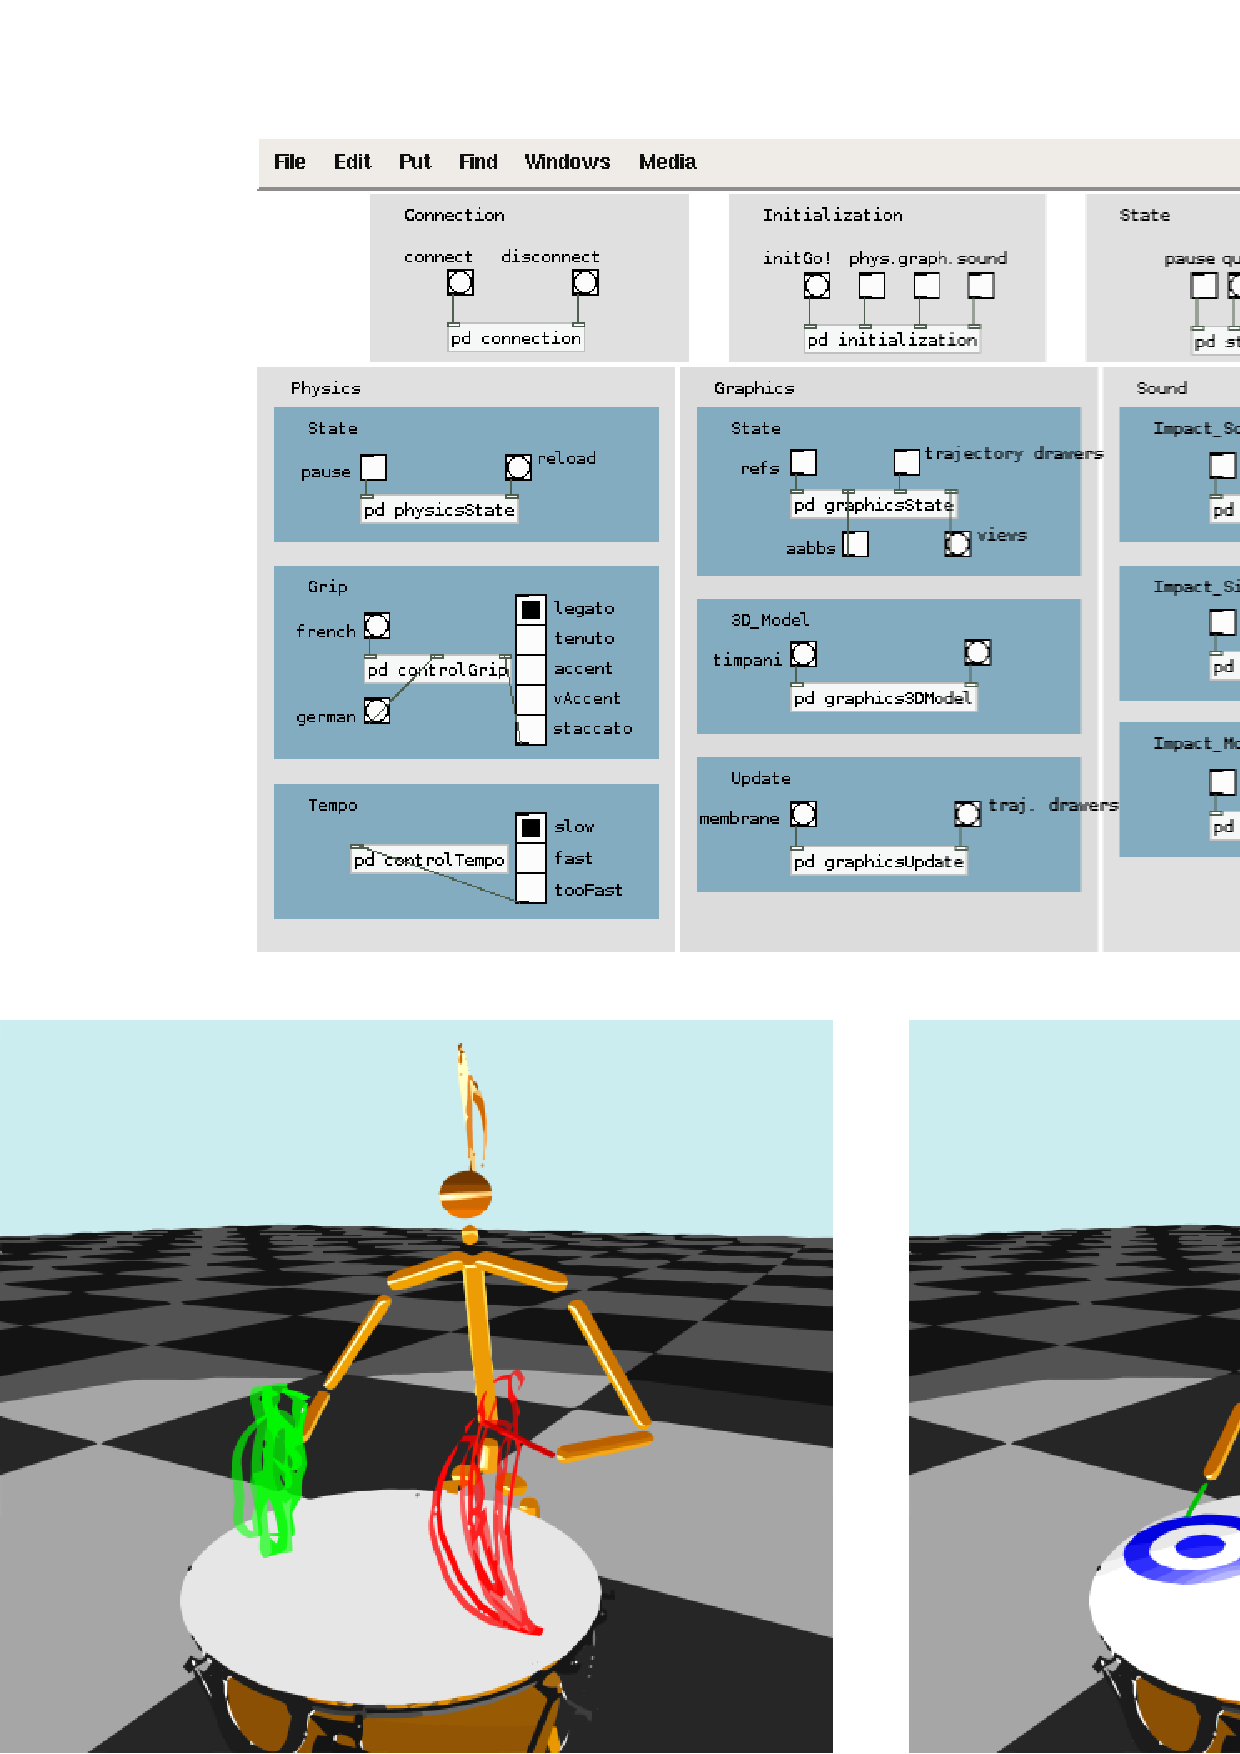
\includegraphics[width=0.8\linewidth]{Chapters/5/Pics/Pdf/userInterface.pdf}
%	\vspace{-0.5cm}
	\caption[User interface]{User interface: users can parameterize the percussion gesture to be simulated (drum grip, playing mode, tempo), as well as the graphics rendering and the sound feedback to be used (sound replay, signal-based and physically-based sound synthesis).}
	\label{fig:userInterface}
\end{figure}

Users can select different percussion grips (\emph{French} or \emph{German}), playing modes (\emph{legato}, \emph{tenuto}, \emph{accent}, \emph{vertical accent} and \emph{staccato}), and different tempi, to be simulated by the virtual percussionist. The parameterization of the visual and sound feedback is also possible. During the simulation, the interface provides users with different sound synthesis models such as the simple playback of sound clips, signal-based sound synthesis, or physics-based sound (modal) synthesis. Every sound synthesis technique proposed by the interface can be tuned in real time. For instance for the modal sound synthesis module, one can tune the parameterization of the drum membrane physics properties (radius size, mass, tension). The available sound and visual feedback is presented in \myfigname \ref{fig:visualFeedback}, which can be parameterized by users with the rendering of helpful visual cues such as mallet trajectories and beat impact locations of the drum membrane.

\begin{figure}[H]
	\begin{center}
		\subfigure[]{\label{fig:sim2}\includegraphics[width=0.3275\linewidth]{Chapters/5/Pics/Pdf/sim-gerard-1}}
		\subfigure[]{\label{fig:sim3}\includegraphics[width=0.3275\linewidth]{Chapters/5/Pics/Pdf/sim-gerard-2}}
		\subfigure[]{\label{fig:sim4}\includegraphics[width=0.3275\linewidth]{Chapters/5/Pics/Pdf/sim-gerard-3}}\\
		\subfigure[]{\label{fig:sim5}\includegraphics[width=0.9\linewidth]{Chapters/5/Pics/Pdf/simSound2}}\\
	\end{center}
	\vspace{-0.5cm}
	\caption[Visual feedback during the simulation]{Visual feedback during the simulation with (a) the final graphical model of the virtual percussionist. Users can explore and visualize the overall virtual percussion performance space, as well as (b) mallet trajectories and (c) beat impact locations. (d) Visual and sound renderings of beat impacts on the drum membrane.}
	\label{fig:visualFeedback}
\end{figure}

%%%%%%%%%%%%%%%%%%%%%%%%%%%%%%%%%%%%%%%%%%%%%%%%%%%%%%%%%%%%%%%%%%%%%%%%%%%%%%%%%%%%%%%%%%%%%%%%%%%%%%%%%%%%%%%%%%%%


%%%%%%%%%%%%%%%%%%%%%%%%%%%%%%%%%%%%%%%%%%%%%%%%%%%%%%%%%%%%%%%%%%%%%%%%%%%%%%%%%%%%%%%%%%%%%%%%%%%%%%%%%%%%%%%%%%%%

	\section{Conclusion}
	\label{sec:Synthesis_Conclusion}

We proposed in this chapter a physically-enabled environment in which a virtual percussionist can be physically controlled and interact with a physics-based sound synthesis model. The physics-based control from real percussion performances guarantees to maintain the main characteristics of human motion data while keeping the physical coherence of the interaction with the simulated instrument.

Furthermore, the hybrid control mode combining \emph{IK} and \emph{ID} controllers leads to a more intuitive and consistent way of editing the motion to be simulated only from mallet extremity trajectories, as regards to the analysis presented in chapter \ref{chapter:Analysis}. This control mode is especially shown to be more accurate than traditional solutions for physically tracking motion capture data. %One limitation of our contribution is however to focus only on upper-body (arms) motion, that does not take into account for instance balance strategies.

Moreover, the proposed asynchronous client-server architecture takes advantage of motion and sound physics formulations, generating in real-time virtual percussion performances that can be parameterized from the motion to the sound. The physical interaction of the virtual percussionist with a physics-based model of a timpani membrane is presented, leading to the control of a sound synthesis model from the actions (impacts) of the virtual percussionist. %It shoulde be noted that this model does not take into account the reaction of gestures as regards to the vibration of the drum membrane.

%Among the perspectives of such work is the improvement of the interaction between motion simulation and sound synthesis. This can involve the design of a more powerful collision detection module. If we consider the physical simulation of the instrument, it might be interesting to include mechanical interactions, such as hammered or plucked interactions, or even modeling the mechanical structure of a finger or a hand. We also plan to extend the mapping possibilities between gesture parameters and sound input parameters, and to develop efficient methods for editing percussion captured motion in the 3D Cartesian space.

%A possible avenue is also to evaluate the musical possibilities offered by our framework for composing novel percussion sequences.



%%%%%%%%%%%%%%%%%%%%%%%%%%%%%%%%%%%%%%%%%%%%%%%%%%%%%%%%%%%%%%%%%%%%%%%%%%%%%%%%%%%%%%%%%%%%%%%%%%%%%%%%%%%%%%%%%%%%



